\subsection{Extracción y Guardado de Segmentos de Audio}

Para esta sección se utiliza el script de MATLAB \texttt{rp1.m}, el cual se adjunta en la entrega.

Se carga el archivo \textit{besh.wav} como vector en MATLAB y se extraen las porciones de la vocal /$\epsilon$/ y la fricativa /sh/. En la figura \ref{fig:p11_extraccion} se muestra el gráfico de la señal \textit{besh.wav} y extracción de las secciones de audio de interés.

\begin{figure}[H]
    \centering
    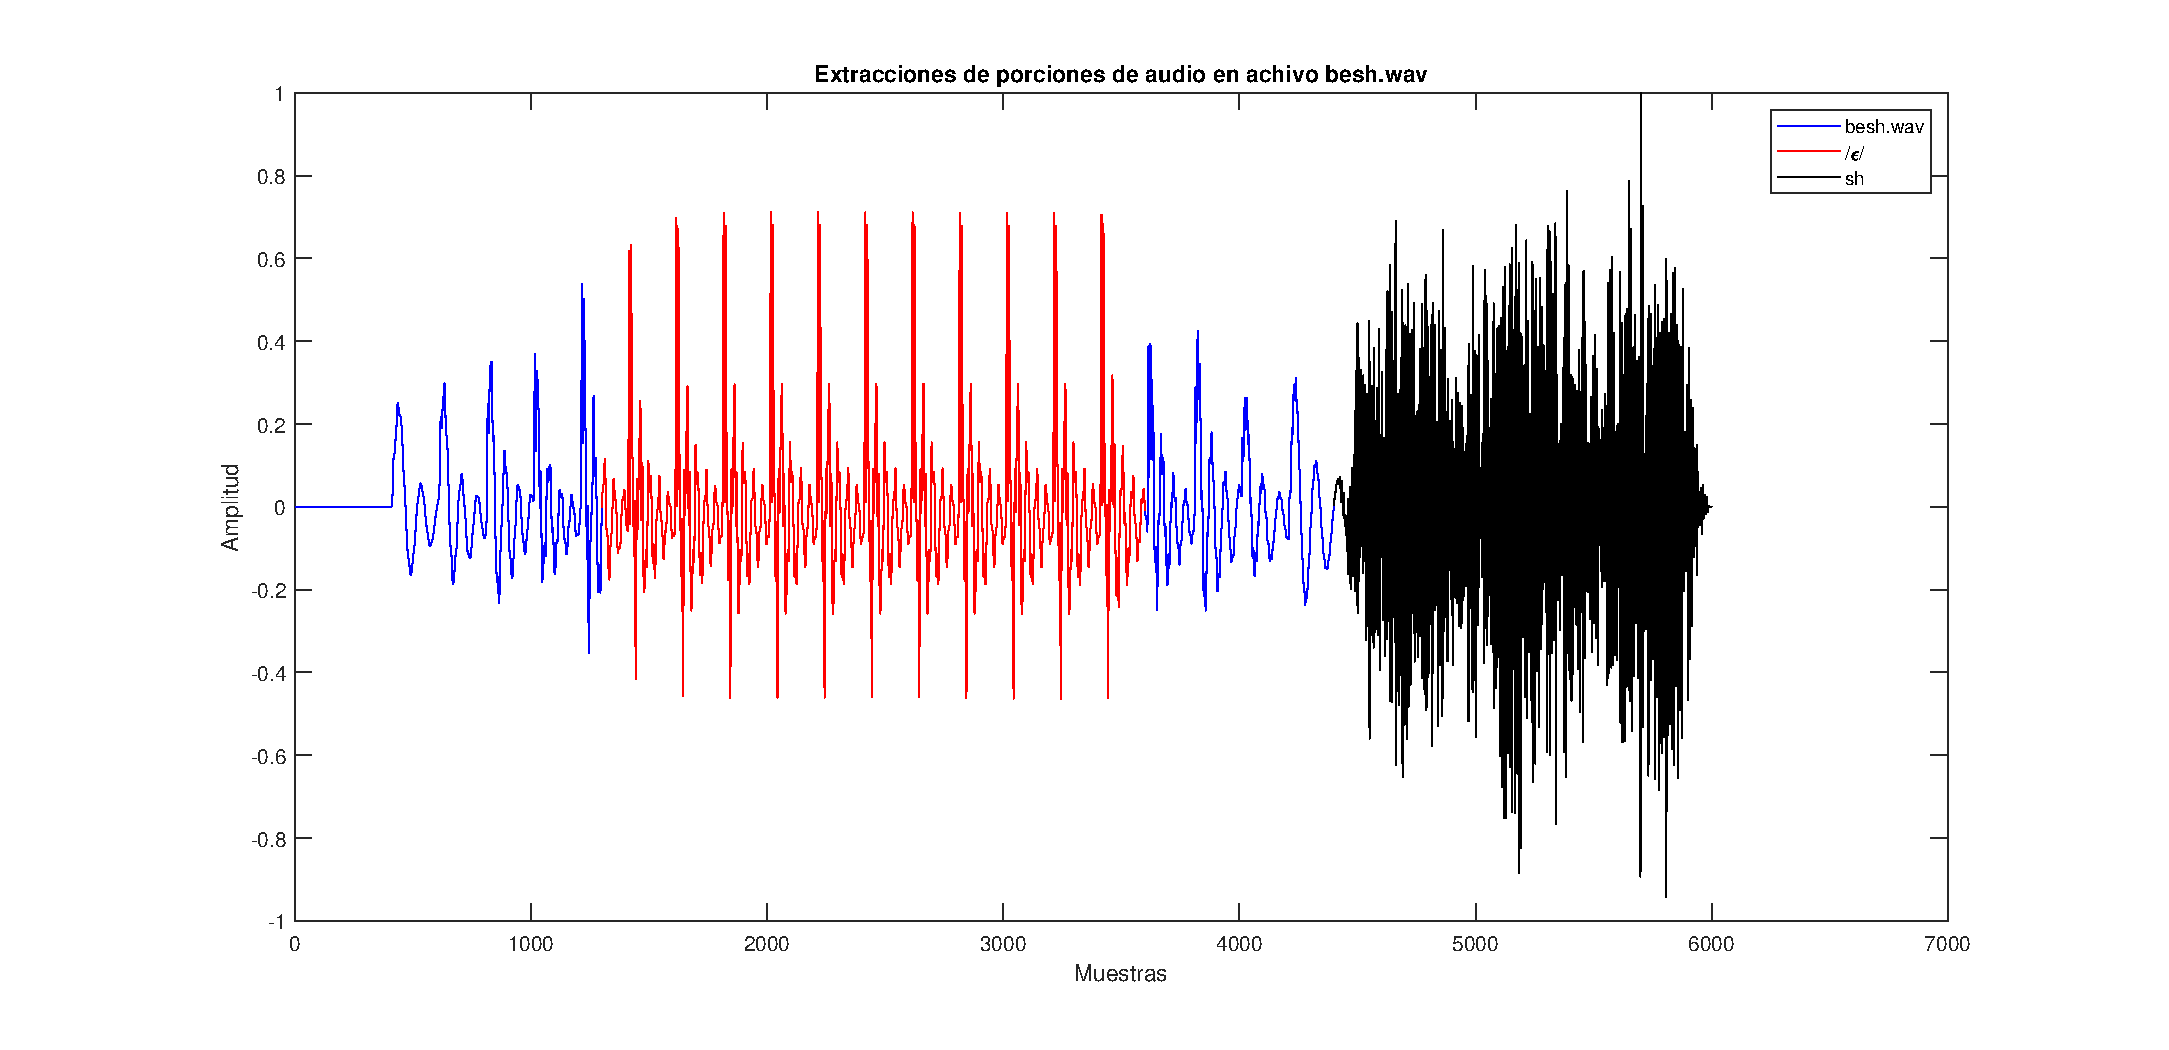
\includegraphics[width = .8\linewidth]{Figuras/p11_extracción.eps}
    \caption{Audio \textit{besh.wav} y extracción de la vocal /$\epsilon$/ y fricativa /sh/.}
    \label{fig:p11_extraccion}
\end{figure}

Se guarda además el segmento de audio correspondiente a la vocal /$\epsilon$/ como \textit{Lab2p1\_vocal.wav} y se adjunta a la entrega.

\subsection{Función en MATLAB para la selección gráfica de un segmento de Audio}

Se escribe la función en MATLAB \texttt{select\_wav} con la cual se selecciona con el mouse un segmento de una señal, se copia dicho segmento en un vector y se guarda en un archivo de audio. La función descrita se muestra a continuación:

\lstinputlisting[language = octave]{Code/select_wav.m}

Se utiliza la función para extraer el segmento de la vocal /$\epsilon$/, quedando guardado en el archivo \textit{lab2p1\_segmento vocal}. Se adjunta dicho archivo a la entrega.